\subsection{Augmented State Machine}
\label{subsec:augment}

To deal with the inherent uncertainty of sniffer traces, we propose to
systematically augment the original monitor state machine with non-deterministic
transitions to account for the difference between the sniffer and DUT traces.

Before formally defining the augmented state machine, we first use an example to
illustrate the basic idea.

\begin{figure}[h!]
  \vspace*{\beforecaptionskip}
  \centering
  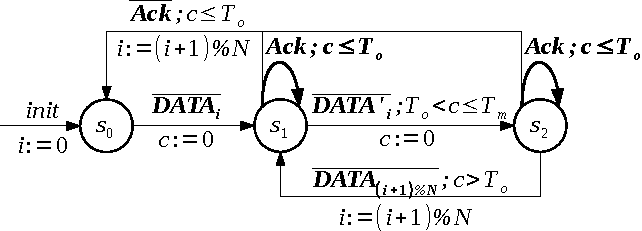
\includegraphics[width=0.7\textwidth]{./figures/dot11_tx_checker.pdf}
  \caption{\textbf{Augmented Monitor State Machine.} Augmented transitions are
  highlighted in bold face. $\overline{Pkt}$ means either $\epsilon$ or $Pkt$.}
  \label{fig:augment}
  \vspace*{\aftercaptionskip}
\end{figure}


Fig.~\ref{fig:augment} shows the augmented state machine for 802.11 transmitter
state machine shown in Fig.~\ref{fig:dot11_tx_ta}.  For each existing transition
(e.g., $s_0\rightarrow s_1$), we add an \textit{empty transition} with same
clock guards and resetting clocks.  This is to account for the possibility when
such packet was observed by the DUT but missed by the sniffer.  Additionally,
for each transition triggered by a \textit{receiving} packet (i.e., $p.dest =
DUT$), such as $s_1\rightarrow s_0$ and $s_2\rightarrow s_0$, we add a
\textit{self transition} with the same trigger packet and clock guards, but
empty set of resetting clocks. This is to allow the state machine make progress
when the sniffer missed such packets.

There are two points worth noticing. First, self transitions are added only for
packets send \textit{to} the DUT, since the sniffer will not overhear packets
\textit{from} the DUT if they were not sent by the DUT. Second, no augmented
transition are added for the packets that are sent to DUT yet are missed by both
the DUT and the sniffer, since such packets do not cause difference between the
DUT and sniffer traces.

The augmented state machine in Fig.~\ref{fig:augment} will accept the sniffer
packet traces $Tr_1$ and $Tr_2$ shown in Fig.~\ref{fig:sniffer_in_middle}.  For
instance, one accepting transition sequence on sniffer trace $Tr_1$ is
$s_0\rightarrow s_1 \rightarrow_s s_1\rightarrow s_2 \rightarrow s_0$, and the
sequence for $Tr_2$ is $s_0 \rightarrow s_1 \rightarrow_e s_2 \rightarrow s_0$,
where $\rightarrow$ is the transition from the original state machine,
$\rightarrow_e$ and $\rightarrow_s$ are the augmented empty and self transitions
respectively.

We now formally define the augmented state machine.

\begin{definition}
  An augmented state machine $S^+$ for a monitor state machine $S$ is a 6-tuple
  $\{\boldsymbol{\Sigma^+}, \mathbb{S}, s_0, C, \boldsymbol{E^+}, G\}$, where $\mathbb{S},
  s_0, C, G$ are the same with $S$. $\Sigma^+=\{\epsilon\} \cup \Sigma$ is
  the augmented input alphabet with the empty symbol, and $E^+ \supset E$ is the
  set of transitions, which includes:
  \begin{itemize}
    \item $E$: existing transitions (\textbf{Type-0}) in $S$.
    \item $E^+_1$: empty transitions (\textbf{Type-1}) for each transition in $E$.
    \item $E^+_2$: self transitions \textbf{(Type-2)} for each transitions
      triggered by receiving packets.
  \end{itemize}
\end{definition}

\begin{comment}
Algorithm~\ref{alg:augment} describes the process of transforming $E$ into
$E^+$.
In particular, Line~\ref{alg:augment:type0} adds existing transitions in $E$ to
$E^+$, while line~\ref{alg:augment:type1} and~\ref{alg:augment:type2} add Type-1
and Type-2 transitions to $E^+$ respectively.

\begin{algorithm}[t!]
  \begin{algorithmic}[1]
    \Function{augment}{$E$}
    \Let{$E^+$}{$\emptyset$}
    \ForAll{$\langle s_i, s_j, p, g, C'\rangle \in E$}
      \Let{$E^+$}{$E^+ \cup \{\langle s_i, s_j, p, g, C'\rangle\}$\Comment{Type-0}}
      \label{alg:augment:type0}
      \Let{$E^+$}{$E^+ \cup \{\langle s_i, s_j, \boldsymbol{\epsilon}, g, C'\rangle\}$\Comment{Type-1}}
      \label{alg:augment:type1}
      \If{$p.dest = DUT$}
        \Let{$E^+$}{$E^+ \cup \{\langle s_i, \boldsymbol{s_i}, p, g, \boldsymbol{\emptyset}\rangle\}$\Comment{Type-2}}
        \label{alg:augment:type2}
      \EndIf
    \EndFor
    \State \Return{$E^+$}
    \EndFunction
  \end{algorithmic}
  \caption{Obtain Augmented Transitions $E^+$ from $E$}
  \label{alg:augment}
\end{algorithm}
\end{comment}

With augmented state machine $S^+$, we can use Type-1 transitions to
non-deterministically infer packets missed by the sniffer, and use Type-2
transitions to consume extra
packets captured by the sniffer but missed by the DUT.

Suppose $P$ is an accepting transition sequence of sniffer trace $Tr$ on the
augmented state machine $S^+$. If we add missed packets indicated by Type-1
transitions to $Tr$, and remove packets indicated by Type-2 transitions from
$Tr$, we obtain a mutation trace $Tr'$, which represents one possibility of the
ground truth---the DUT packet trace.

In fact, we show that Problem~\ref{prob:validation} is equivalent to the
satisfiability problem of $Tr$ on $S^+$.

\begin{theorem}
  There exists a mutation trace $Tr' \in \mathcal{M}(Tr)$ that satisfies $S$ if
  and only if $Tr$ satisfies $S^+$.
 \label{the:equivalent}
\end{theorem}

By Theorem~\ref{the:equivalent}, the inherent uncertainty of the sniffer traces
are explicitly represented by the augmented transitions, and can be
systematically explored using the well established state machine theory.

One immediate observation can be drawn from Theorem~\ref{the:equivalent} by
contradiction.

\begin{corollary}
  If $S^+$ rejects $Tr$, then $S$ rejects $Tr_{DUT}$.
  \label{cor:false_pos}
\end{corollary}
In the context of validation where we raise a violation alarm when $S^+$
rejects $Tr$, Corollary~\ref{cor:false_pos} guarantees that no false alarms will be
raised.
However, when $S^+$ accepts $Tr$, $S$ could still reject $Tr_{DUT}$.
In other words, the conclusion of the validation can either be \textit{definitely
wrong} or \textit{possibly correct}, but not \textit{definitely correct}.
This is the fundamental limitation caused by the uncertainty of sniffer traces.
